\section*{Results and Analysis}
\label{Results}
The data from \textit{Men and Bread} is analysed using PCA and the results from the analysis will be presented in the following section.\blankline
%
%Analyze the results from the example using PCA.
%First plot a “profile” of all stimuli.
%
The profile plot is made based on the mean attribute ratings of every test subject. The attributes are listed on the x-axis and the rating on the y-axis. A profile for each bread has been plotted together, see \autoref{fig:plot}. The profile plot gives an overview of how the different bread compare to each other. E.g. \textit{Bread 1} was rated as the highest on the attribute "Krumme" whereas it appears that the test subjects somewhat all agreed on the attribute "Saftigt".
%
\begin{figure}[H]
\centering
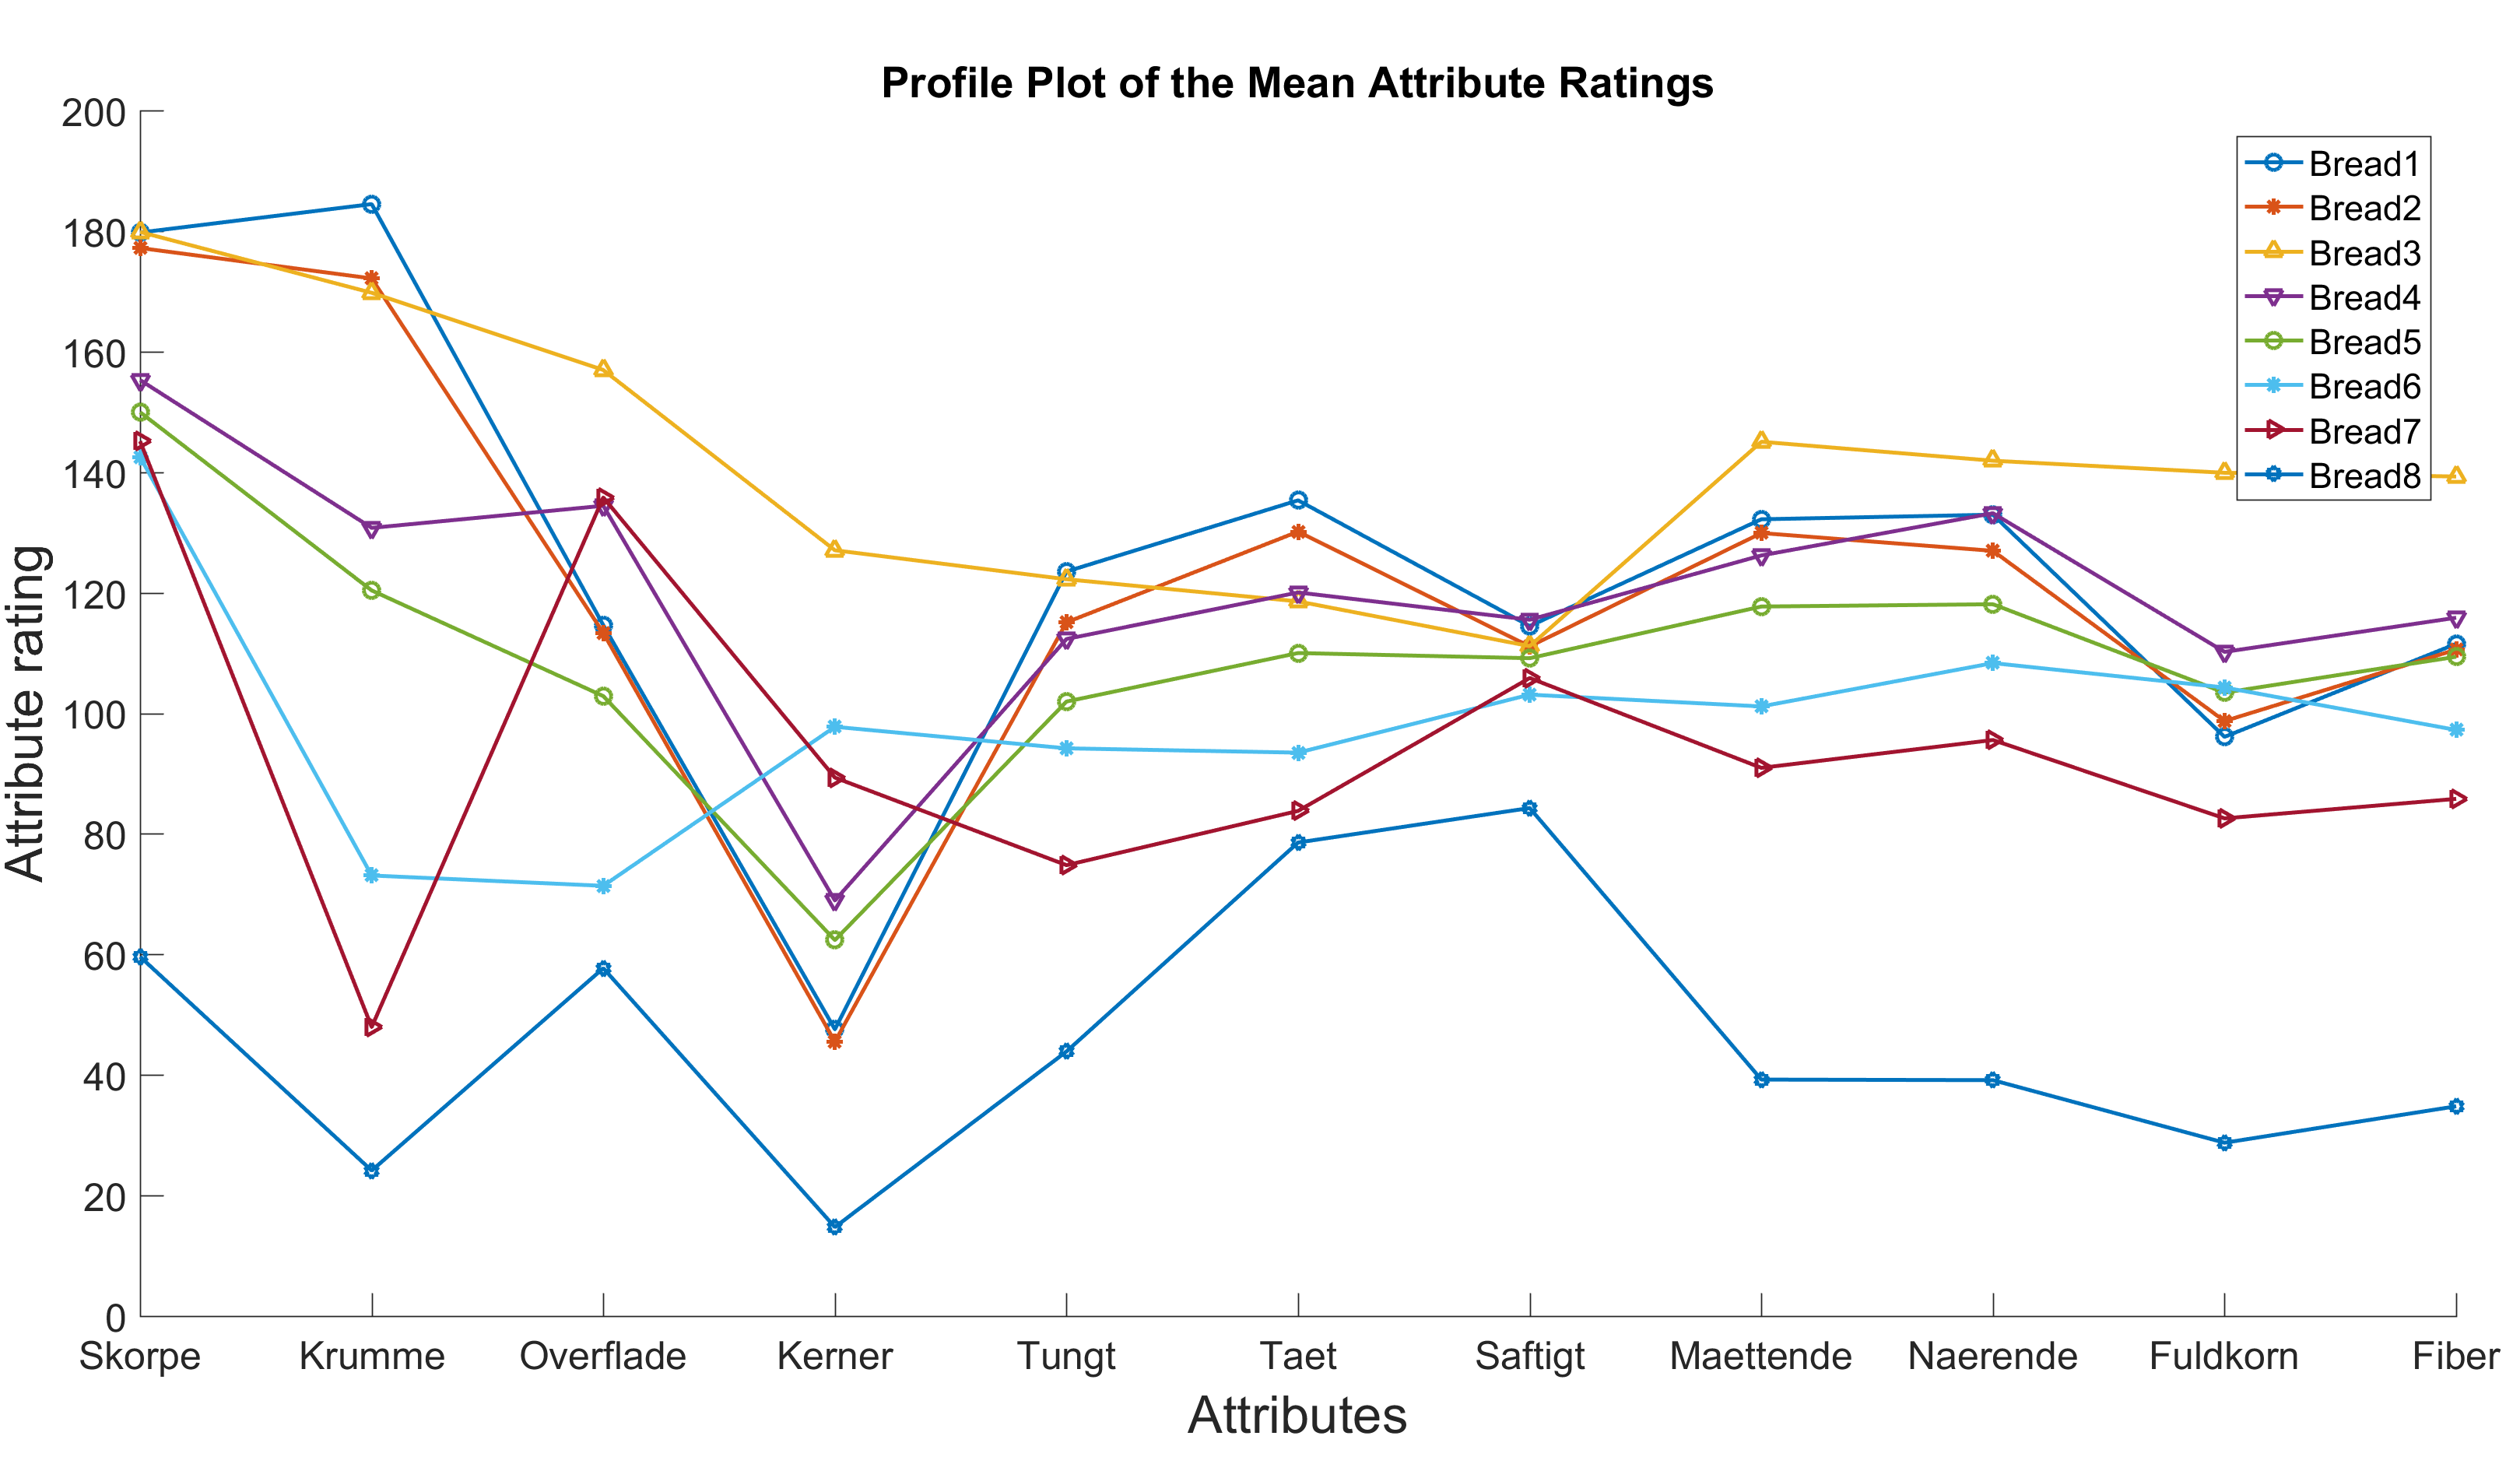
\includegraphics[width=\textwidth]{Figure/profile_plot.png}
\caption{A profile plot of all the mean attribute values as rated by the test subjects. All 8 bread-types are listed in the legend. Bread 1 received the highest average rating in the attribute "Krumme".}
\label{fig:plot}
\end{figure}
\noindent
%
%How much of the variance is explained by each component?
%(Plot a scree-plot including cumulative variance).
%
In \autoref{tab:explained} the variance explained by each of the first seven principal components are presented. It is shown that 81.04 \% of the variance is explained by PC1, 13.61 \% by PC2 and 3.31 \% by PC3. 
%
\begin{table}[H]
\centering
\begin{tabular}{lc}
\hline
                         & \multicolumn{1}{l}{Variance Explained (\%)} \\ \hline
\multicolumn{1}{l|}{PC1} & 81.04                                       \\
\multicolumn{1}{l|}{PC2} & 13.61                                       \\
\multicolumn{1}{l|}{PC3} & 3.31                                        \\
\multicolumn{1}{l|}{PC4} & 1.28                                        \\
\multicolumn{1}{l|}{PC5} & 0.65                                        \\
\multicolumn{1}{l|}{PC6} & 0.10                                        \\
\multicolumn{1}{l|}{PC7} & 0.01                                       
\end{tabular}
\caption{Explained variance by each principal component.}
\label{tab:explained}
\end{table}
\noindent
%
To get an overview of the number of PC according to how much of the variance they explain, the explained variance from each principal component is plotted in a barplot and an accumulative scree-plot, see \autoref{fig:scree}. On the scree-plot in \autoref{fig:scree}, there is a knee point at PC2 and it is therefore chosen to use two principal components in the analysis. In total 94.65 \% of the variance is explained by the two principal components.
%
\begin{figure}[H]
\centering
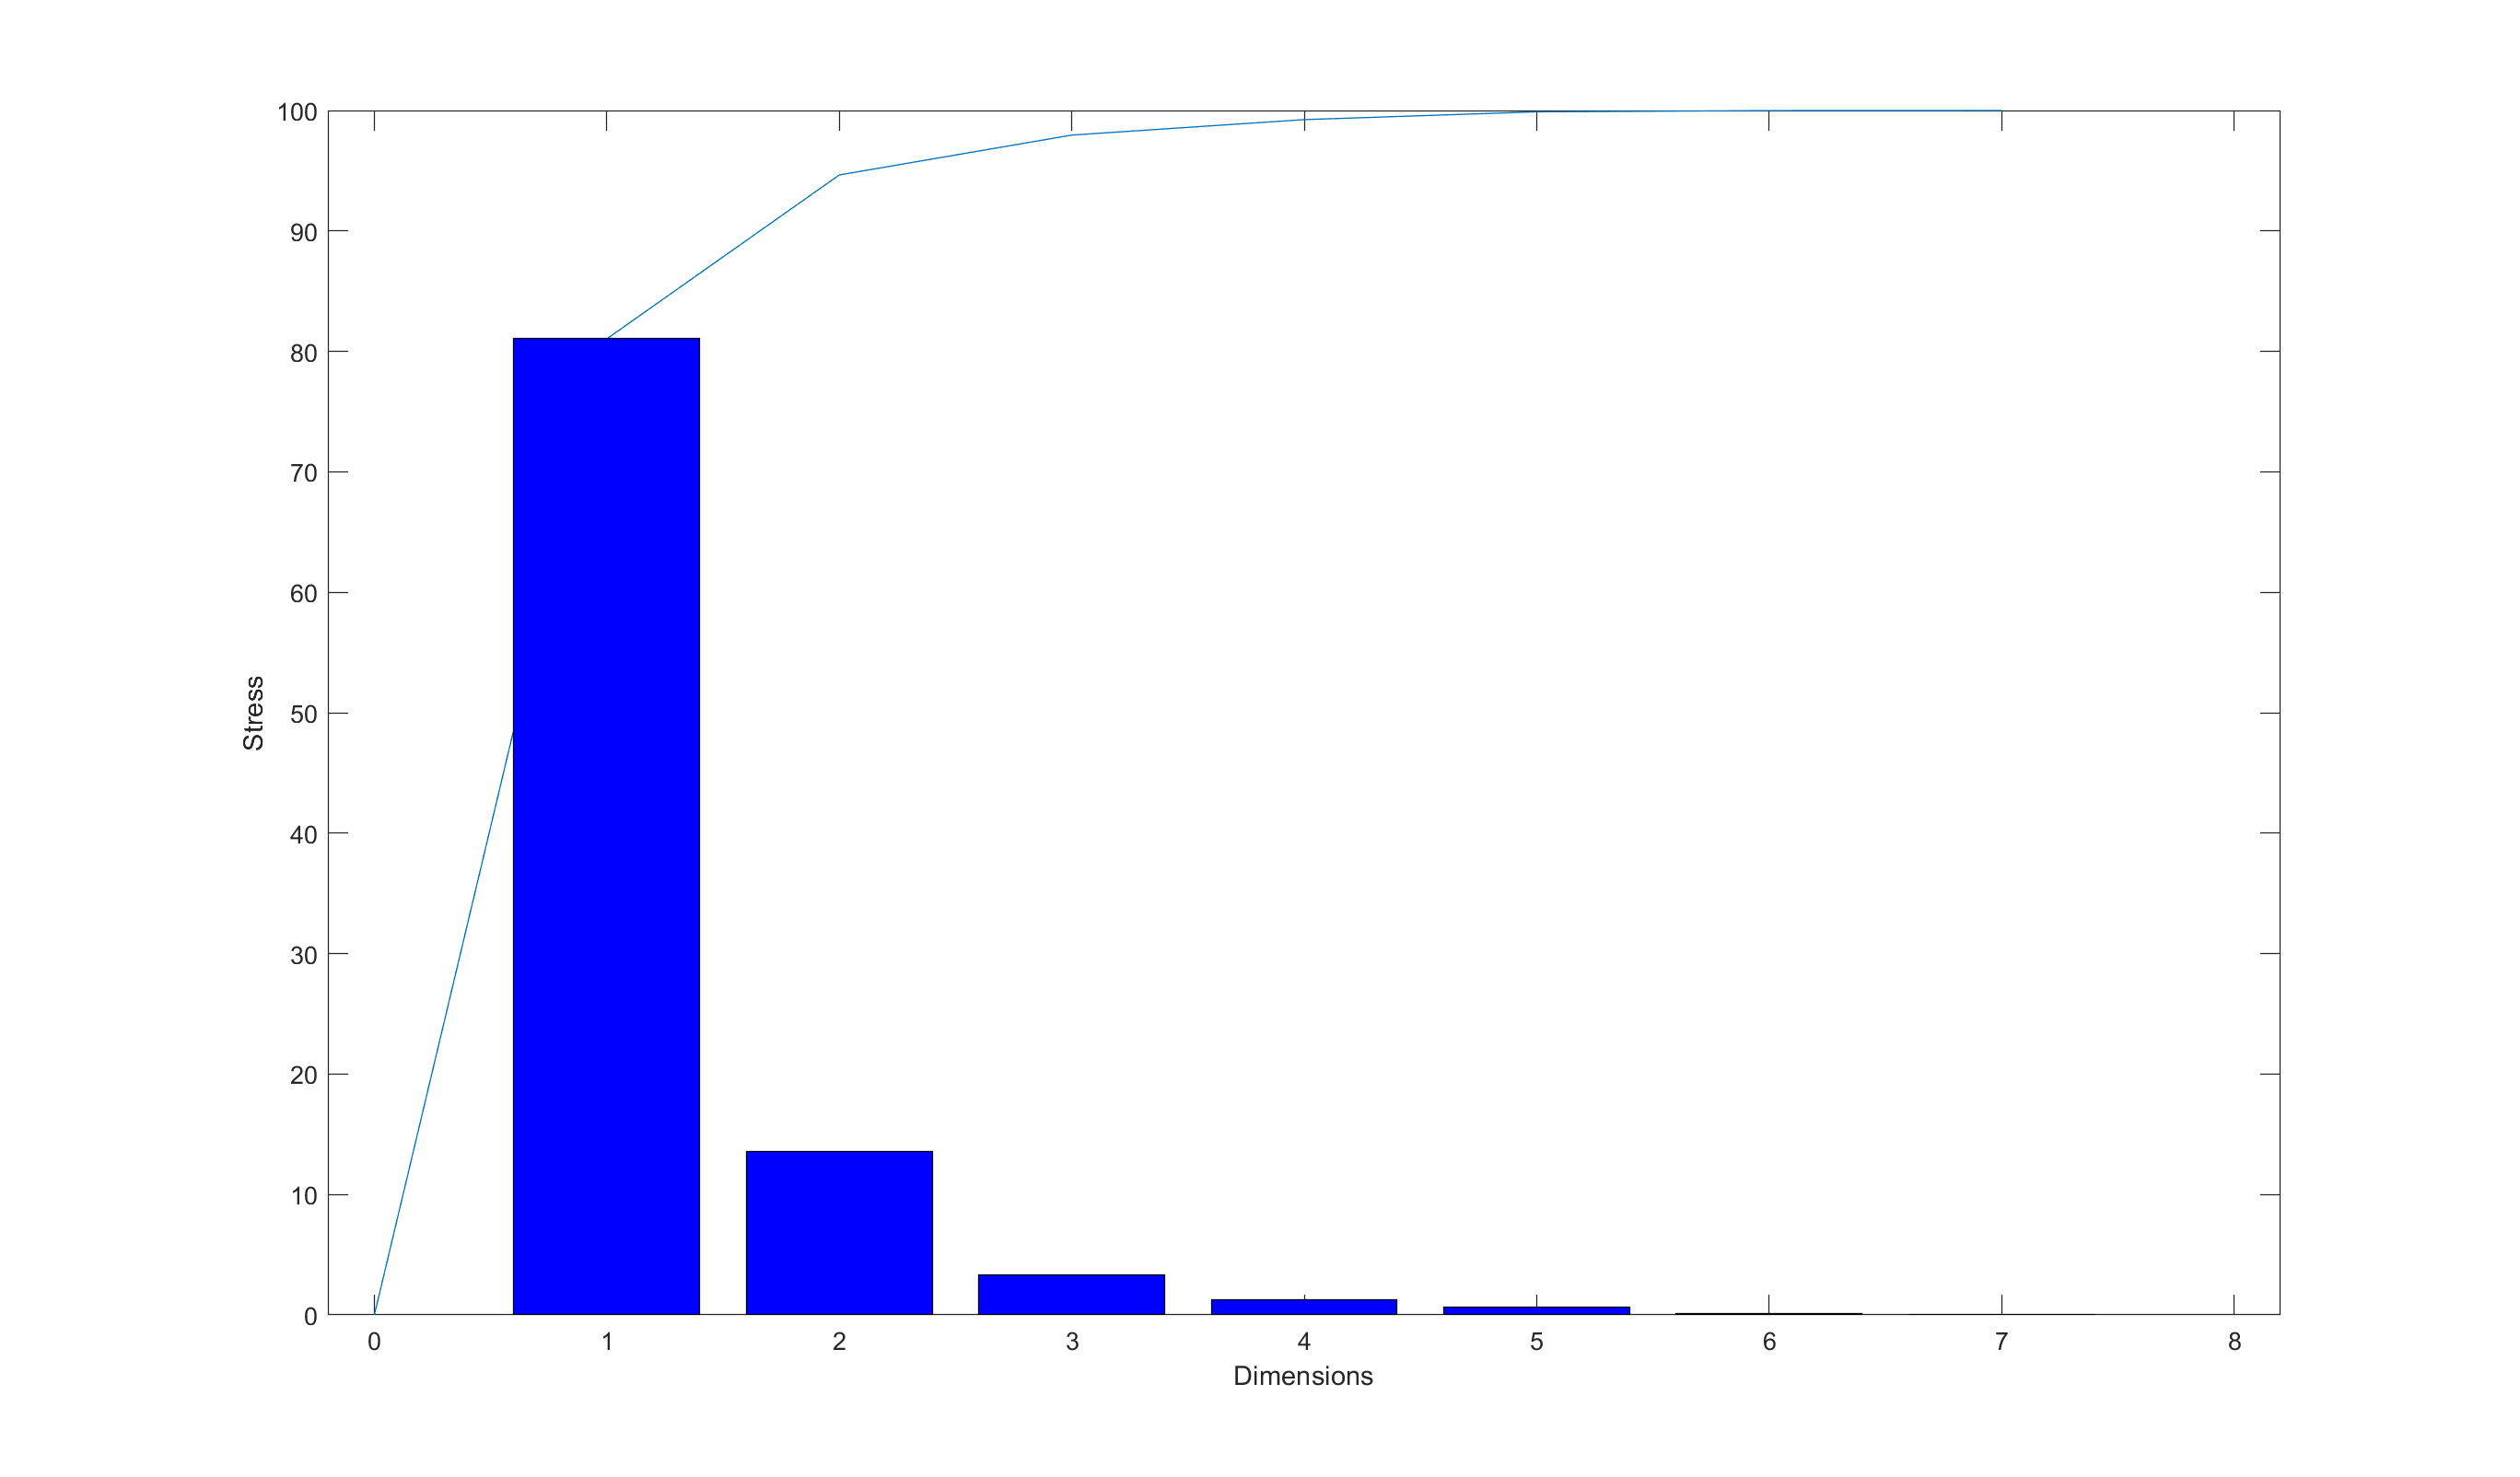
\includegraphics[width =\textwidth]{Figure/Screeplot}
\caption{Accumulative scree plot and barplot showing how much of the variance is explained by each principal component.}
\label{fig:scree}
\end{figure}
\noindent
%
%Plot your PCA solution graphically. Both a plot with just your stimuli (scores) and a biplot with both scores and loadings.
%
The principal component analysis is conducted. The first plot from the analysis is presented on \autoref{fig:scoreplot}, which is a score plot with two dimensions. \blankline
%
From the score-plot it is apparent that B1 and B2 are placed close together and they therefore share similar overall properties, based on this plot. B4 and B5 also have quite similar properties, as well as B6 and B7. Both B8 and B3 are very different from all the other buns.
\newpage
%
\begin{figure}[H]
\centering
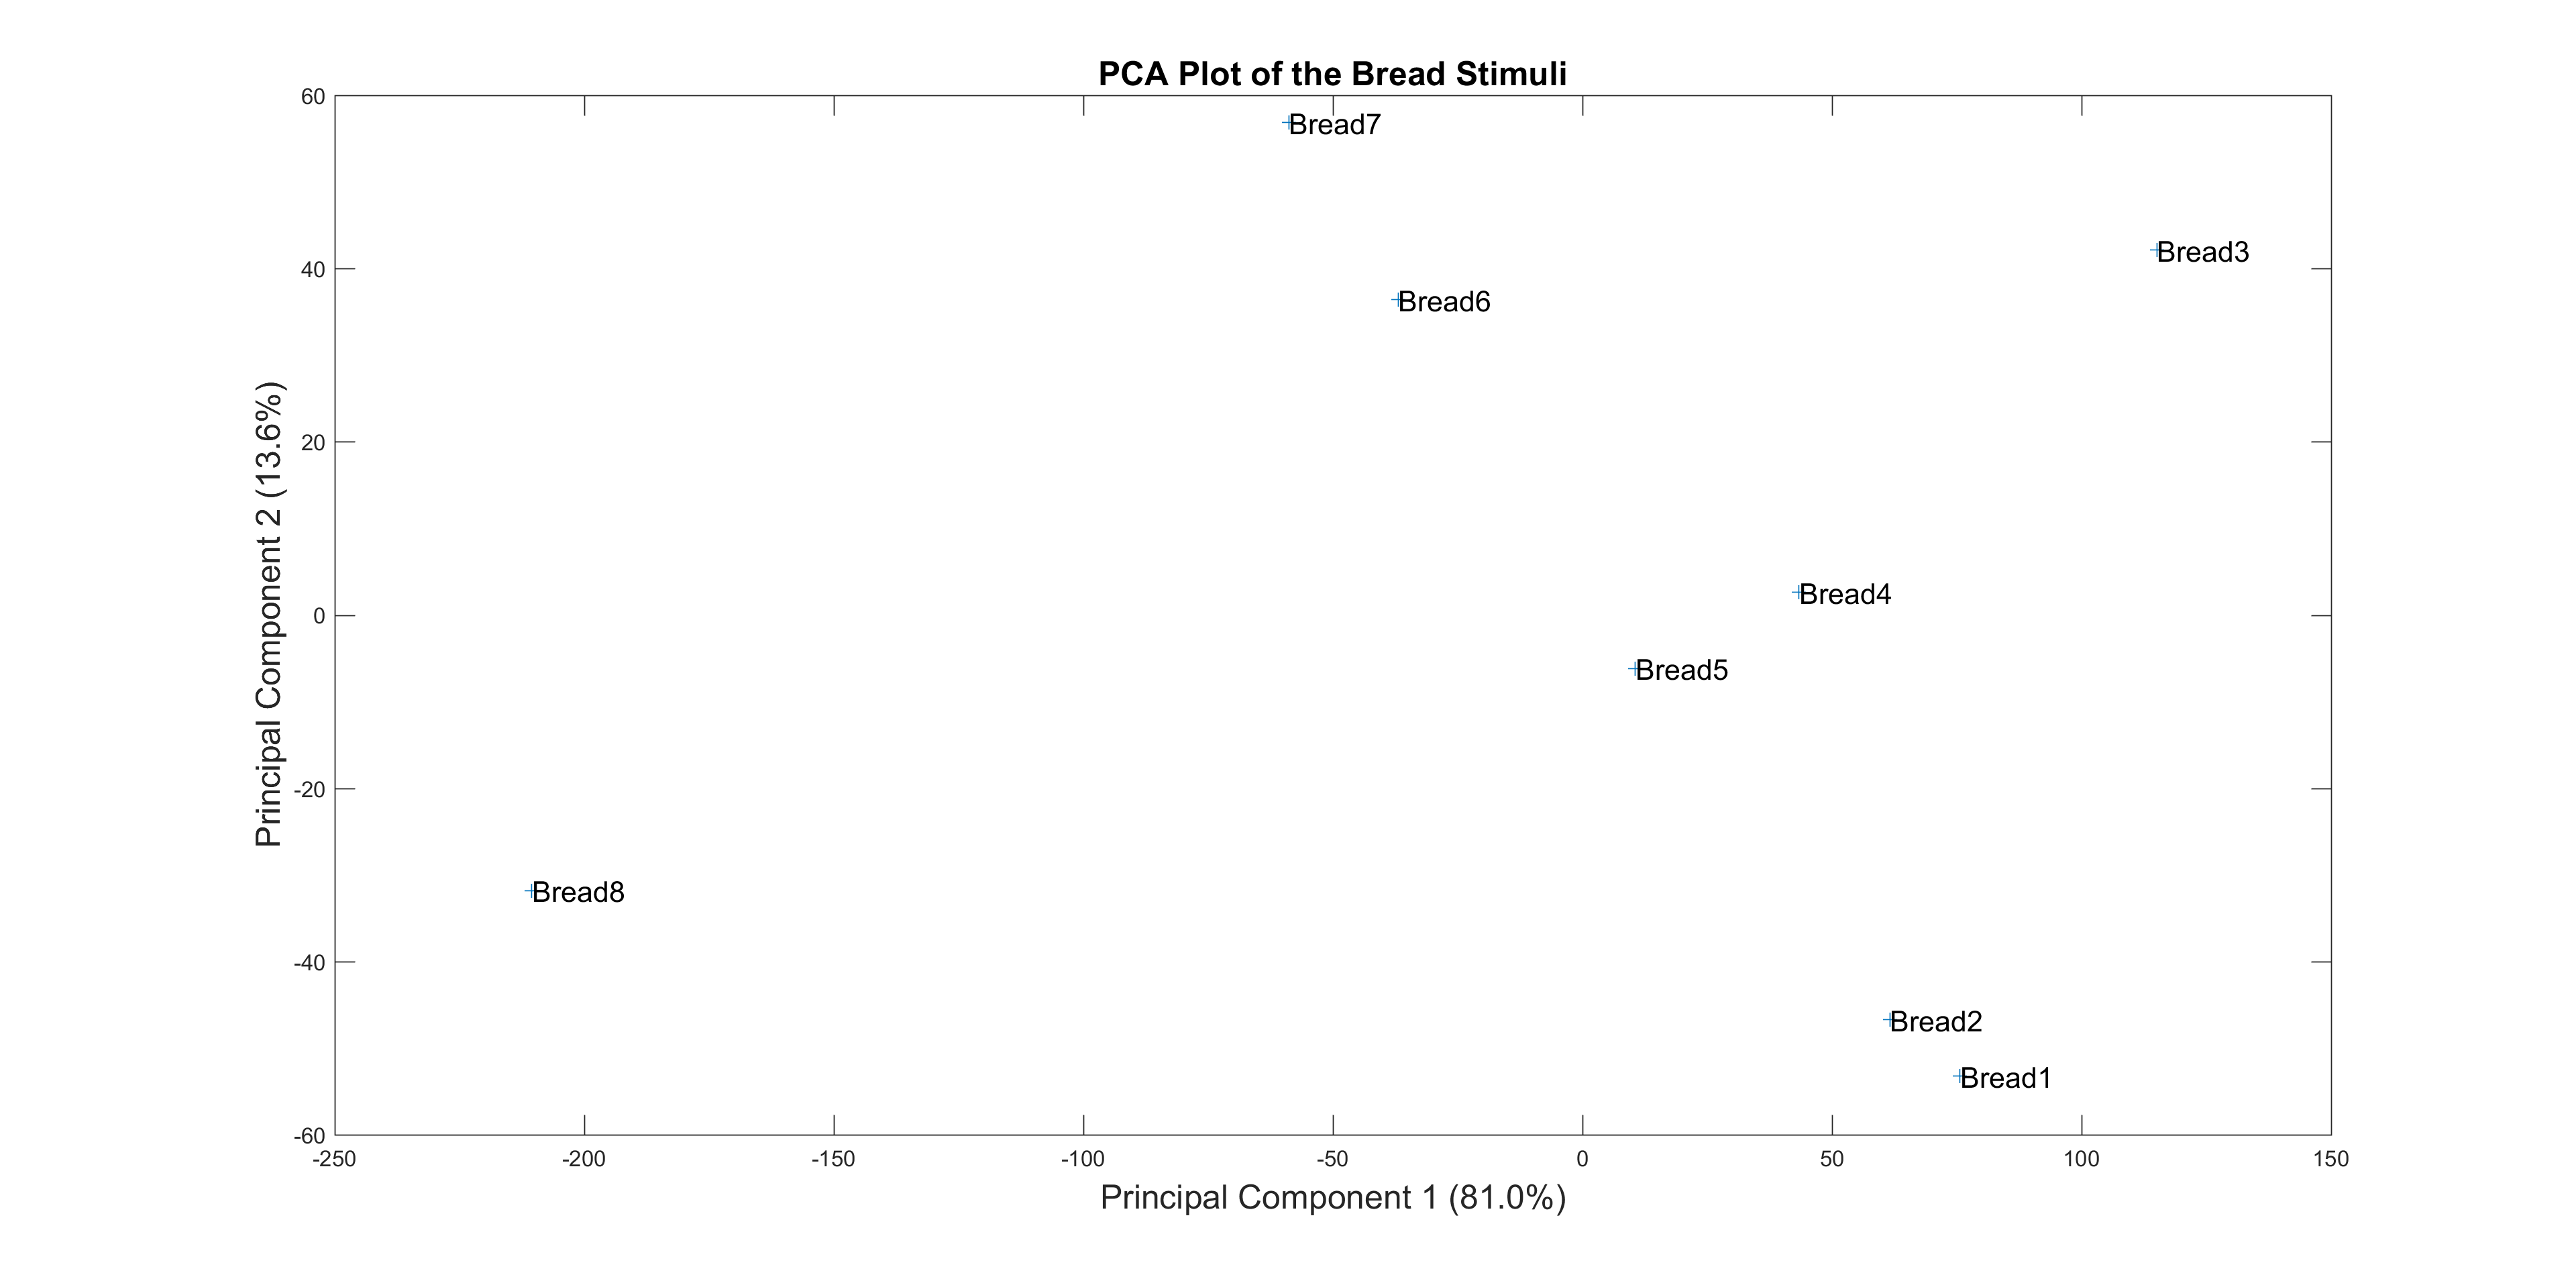
\includegraphics[width =\textwidth]{Figure/PCA_plot}
\caption{PCA score plot in two dimensions.}
\label{fig:scoreplot}
\end{figure}
\noindent 
%
The next plot is presented on \autoref{fig:biplot} where both the scores and loading values are plotted in a bi-plot. 
%
\begin{figure}[H]
\centering
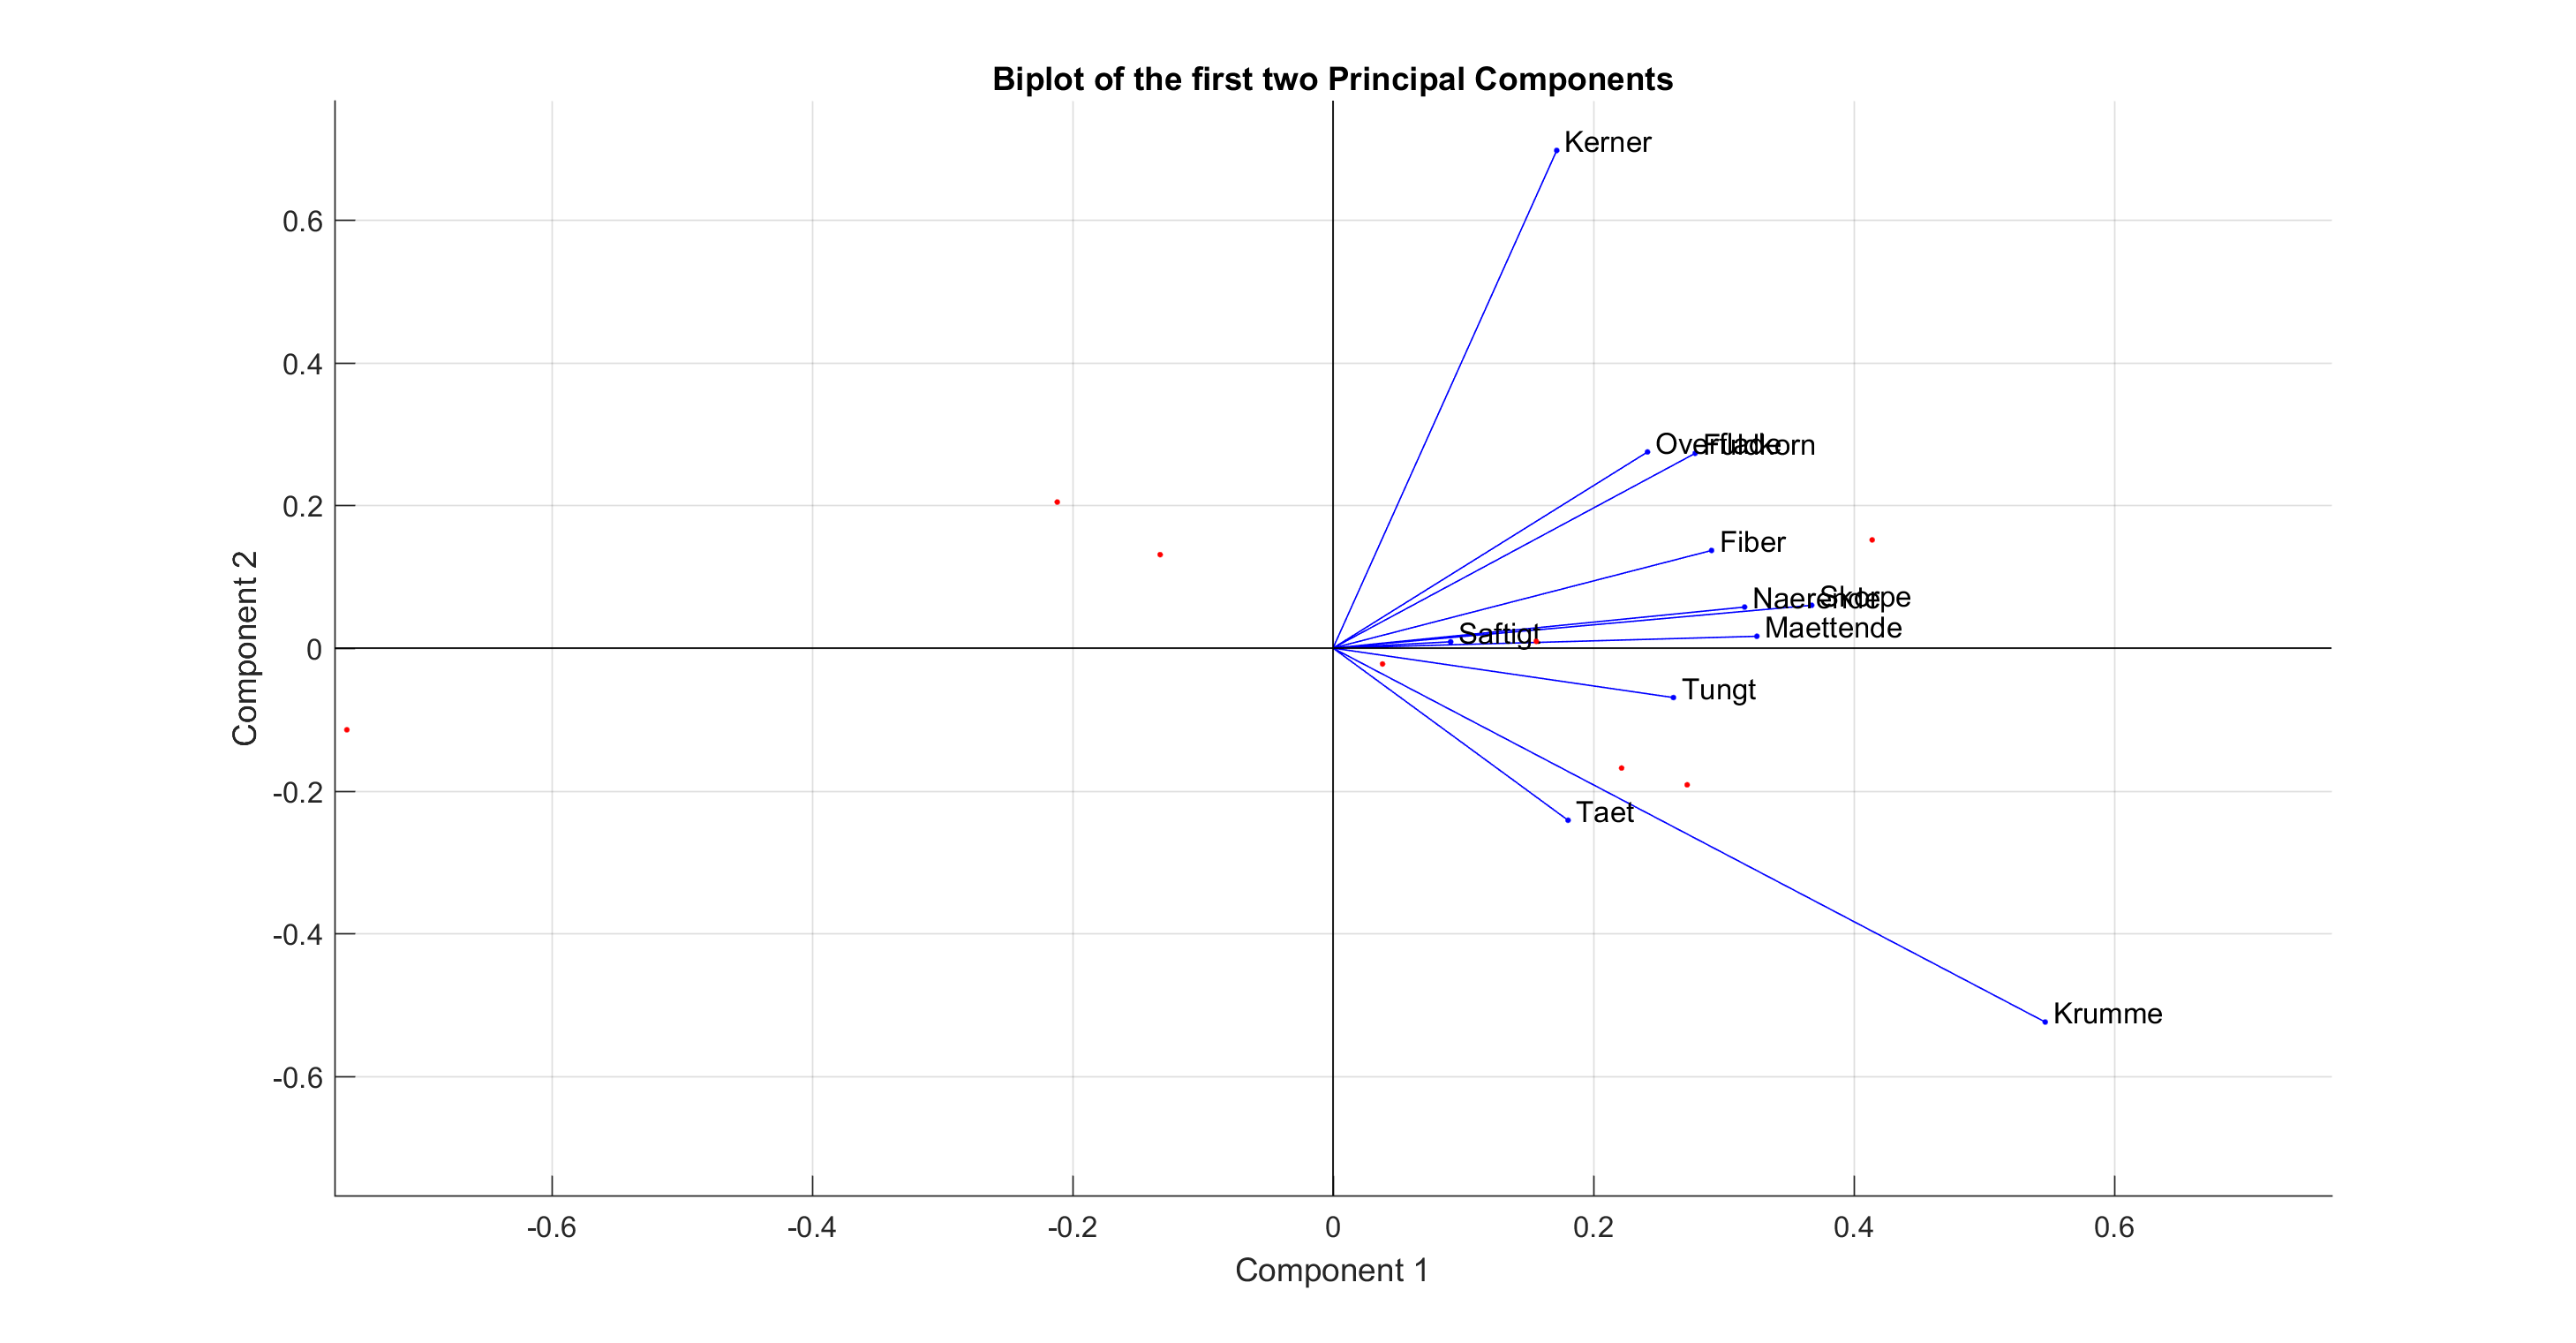
\includegraphics[width =\textwidth]{Figure/biplot}
\caption{Biplot with both score and loading values. The red marks represent the score values and the blue lines represent the loading values.}
\label{fig:biplot}
\end{figure}
\noindent
%
The bi-plot shows that "Krumme" contributes to most of the PC1 and "Kerner" contributes to most of the PC2. "Saftig" doesn't really contribute that much to any of the two principal components.
None of the variables are placed on different sides of the origin compared to each other and therefore none of the variables seems to be negatively correlated. \blankline
%Make a table of the loadings of each word-pair on each principal component.
A table with the loadings of each word-pair on each of the first seven principal components are presented in \autoref{tab:loadings}.
%
\begin{table}[H]
\centering
\begin{tabular}{llllllll}
\hline
\textbf{}                               & \textbf{PC1}    & \textbf{PC2}    & \textbf{PC3}    & \textbf{PC4}    & \textbf{PC5} & \textbf{PC6} & \textbf{PC7} \\ \hline
\multicolumn{1}{l|}{\textbf{Skorpe}}    & 0.3678          & 0.0600          & -0.0046         & \textbf{0.6897} & 0.5477       & -0.1959      & 0.1392       \\
\multicolumn{1}{l|}{\textbf{Krumme}}    & \textbf{0.5472} & -0.5240         & 0.0189          & -0.4872         & 0.3211       & -0.0521      & -0.1313      \\
\multicolumn{1}{l|}{\textbf{Overflade}} & 0.2416          & 0.2748          & \textbf{0.9111} & -0.0847         & -0.1001      & 0.0329       & 0.0650       \\
\multicolumn{1}{l|}{\textbf{Kerner}}    & 0.1719          & \textbf{0.6974} & -0.2236         & -0.3361         & 0.4033       & 0.3256       & -0.0727      \\
\multicolumn{1}{l|}{\textbf{Tungt}}     & 0.2616          & -0.0693         & -0-1562         & 0.0663          & -0.1392      & 0.4939       & -0.1535      \\
\multicolumn{1}{l|}{\textbf{Tæt}}       & 0.1806          & -0.2413         & 0.0132          & 0.0035          & -0.1153      & 0.3682       & 0.5569       \\
\multicolumn{1}{l|}{\textbf{Saftigt}}   & 0.0904          & 0.0088          & 0.0413          & 0.2347          & -0.1858      & 0.1851       & -0.4137      \\
\multicolumn{1}{l|}{\textbf{Mættende}}  & 0.3257          & 0.0166          & -0.0613         & 0.0962          & -0.1729      & -0.2379      & -0.0712      \\
\multicolumn{1}{l|}{\textbf{Nærende}}   & 0.3163          & 0.0575          & -0.1049         & 0.2613          & -0.3638      & 0.3427       & -0.0214      \\
\multicolumn{1}{l|}{\textbf{Fuldkorn}}  & 0.2783          & 0.2729          & -0.2608         & -0.1629         & -0.3320      & -0.3433      & 0.5211       \\
\multicolumn{1}{l|}{\textbf{Fiber}}     & 0.2908          & 0.1368          & -0.1029         & -0.0573         & -0.2907      & -0.3823      & -0.4148     
\end{tabular}
\caption{Loadings of each word-pair on each of the first seven principal components. Values in bold indicates high load and therefore contributes to most of the PC.}
\label{tab:loadings}
\end{table}
%
%Interpret the solution. Also, are there word-pairs that seem ”redundant” e.g. measures that same perceptual attribute?
%
\begin{figure}[H]
\centering
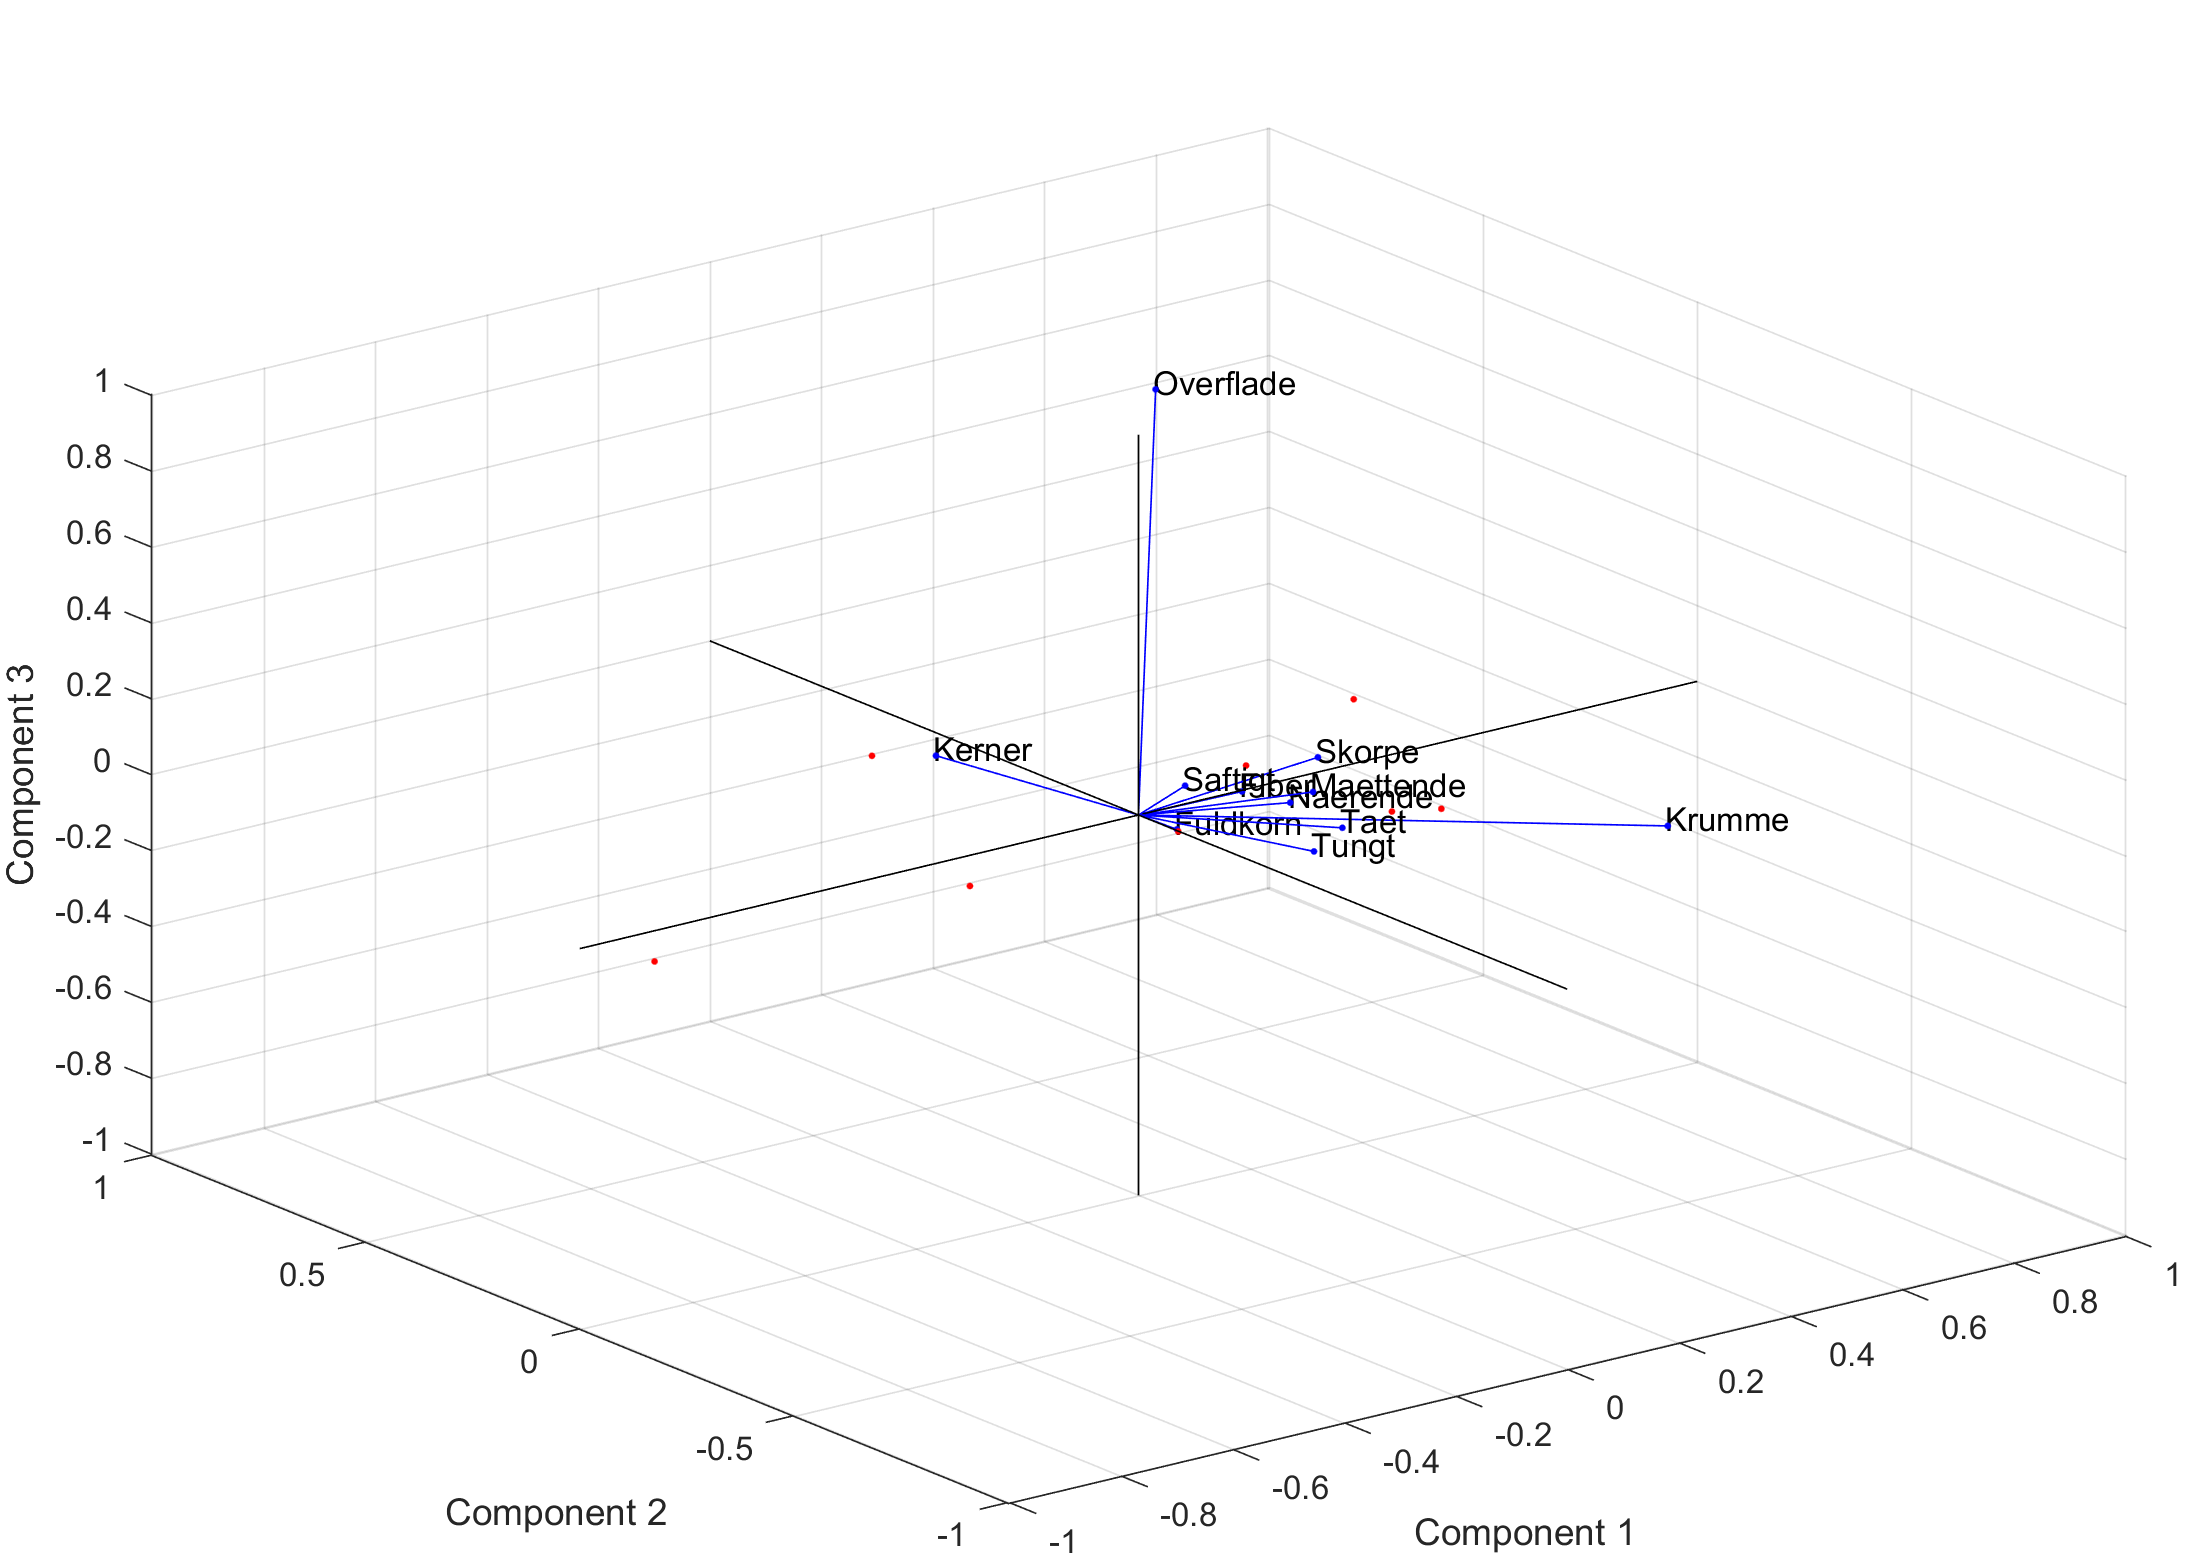
\includegraphics[width =\textwidth]{Figure/biplot_3D_std}
\caption{Bi-plot in three dimensions.}
\label{fig:3Dbiplot}
\end{figure}
\noindent
%
Based on \autoref{fig:biplot}, it looks like "Overflade" and "Fuldkorn" are highly correlated, but after looking at the 3D bi-plot, \autoref{fig:3Dbiplot}, it is clear that "Overflade" and "Fuldkorn" are actually quite different. From this plot, we can see that the attribute "Overflade" explains most of the PC3, since it is almost the only attribute that deviates in the third dimension. This is confirmed by the loadings presented in \autoref{tab:loadings}, where 91.1 \% of PC3 is explained by "Overflade".\blankline
%
From \autoref{fig:biplot}, it also looks like "Nærende", "Mættende", and "Skorpe" are highly correlated, which is confirmed by the 3D biplot on \autoref{fig:3Dcorrelation}. Therefore, some of these three attributes might be redundant. 
%
\begin{figure}[H]
\centering
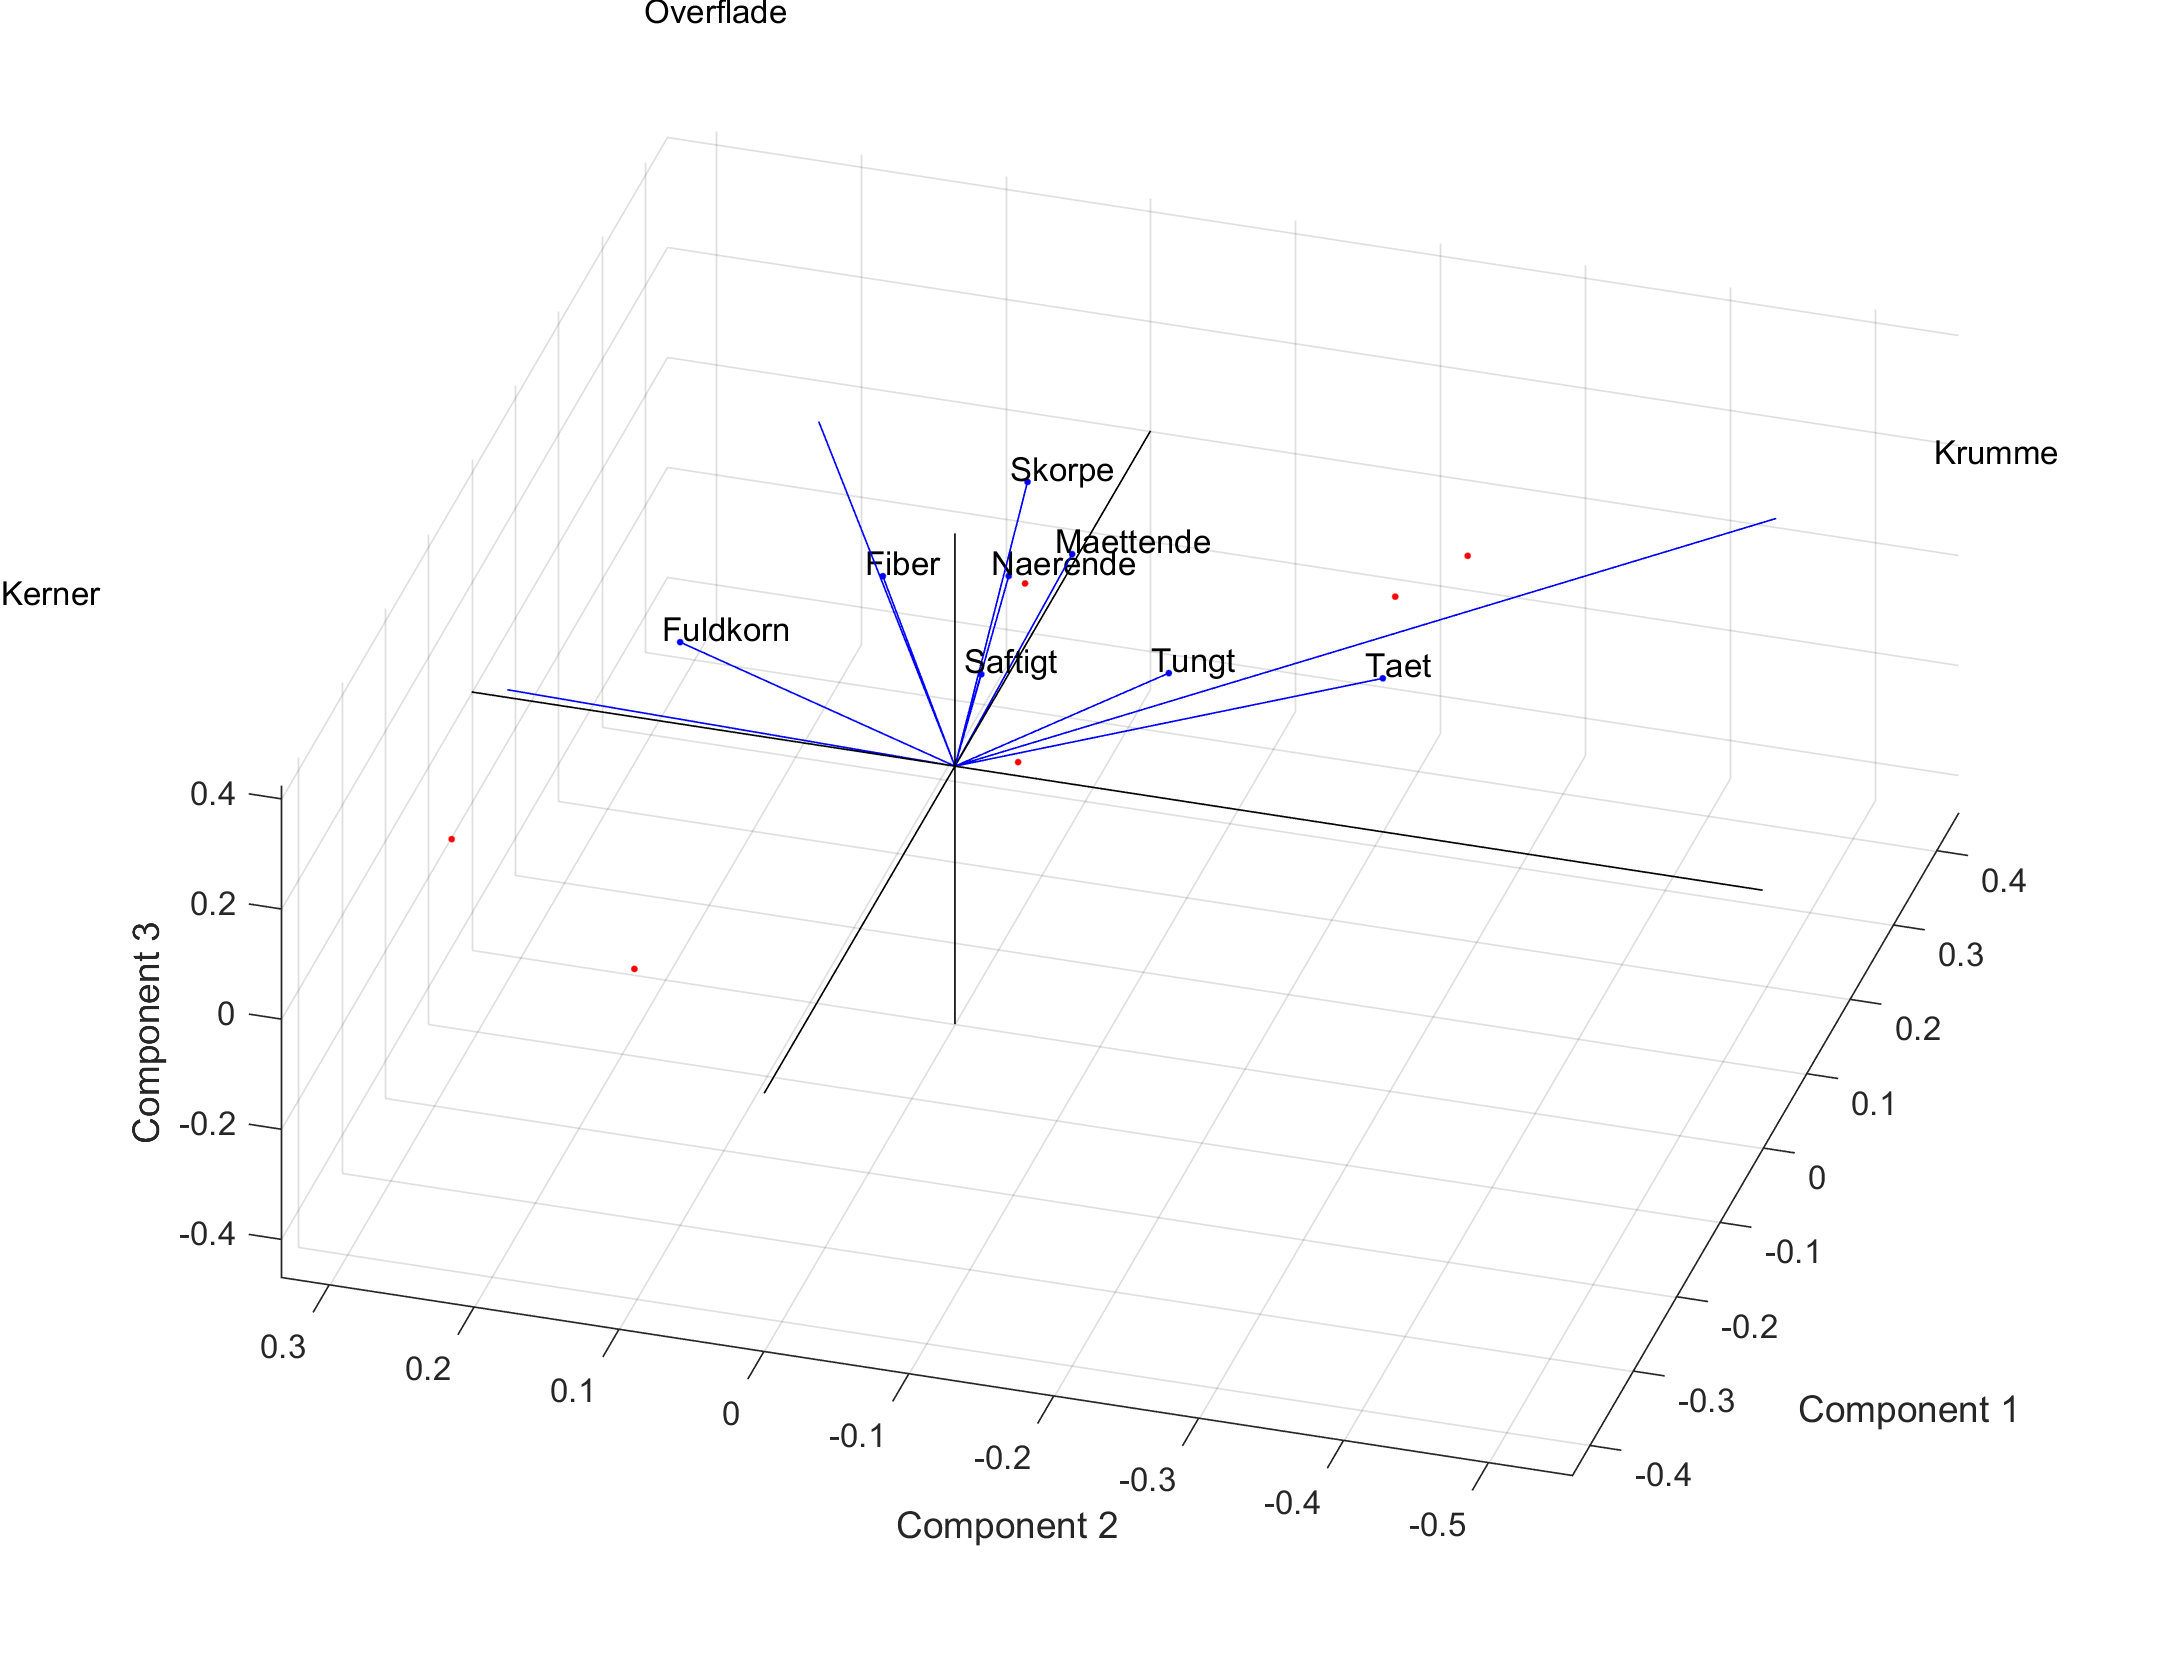
\includegraphics[width =\textwidth]{Figure/biplot_3D_maet}
\caption{Bi-plot in three dimensions, same as \autoref{fig:3Dbiplot}, just from another angle.}
\label{fig:3Dcorrelation}
\end{figure}
\noindent
%
The attribute "Saftig" doesn't really contribute to any of the three principal components and according to \autoref{fig:plot} the rating of this attribute doesn't vary that much between the different buns which also indicates that this attribute isn't that important for this PCA.